
\let\negmedspace\undefined
\let\negthickspace\undefined
\documentclass[journal]{IEEEtran}
\usepackage[a5paper, margin=10mm, onecolumn]{geometry}
%\usepackage{lmodern} % Ensure lmodern is loaded for pdflatex
\usepackage{tfrupee} % Include tfrupee package

\setlength{\headheight}{1cm} % Set the height of the header box
\setlength{\headsep}{0mm}     % Set the distance between the header box and the top of the text

\usepackage{gvv-book}
\usepackage{gvv}
\usepackage{cite}
\usepackage{amsmath,amssymb,amsfonts,amsthm}
\usepackage{amsmath}
\usepackage{algorithmic}
\usepackage{graphicx}
\usepackage{textcomp}
\usepackage{xcolor}
\usepackage{txfonts}
\usepackage{listings}
\usepackage{enumitem}
\usepackage{mathtools}
\usepackage{gensymb}
\usepackage{comment}
\usepackage[breaklinks=true]{hyperref}
\usepackage{tkz-euclide} 
\usepackage{listings}
% \usepackage{gvv}                                        
\def\inputGnumericTable{}                                 
\usepackage[latin1]{inputenc}                                
\usepackage{color}                                            
\usepackage{array}                                            
\usepackage{longtable}                                       
\usepackage{calc}                                             
\usepackage{multirow}                                         
\usepackage{hhline}                                           
\usepackage{ifthen}                                           
\usepackage{lscape}
\usepackage{circuitikz}
\tikzstyle{block} = [rectangle, draw, fill=blue!20, 
    text width=4em, text centered, rounded corners, minimum height=3em]
\tikzstyle{sum} = [draw, fill=blue!10, circle, minimum size=1cm, node distance=1.5cm]
\tikzstyle{input} = [coordinate]
\tikzstyle{output} = [coordinate]


\begin{document}

\bibliographystyle{IEEEtran}
\vspace{3cm}

\title{5.3.12}
\author{AI25BTECH11018-Hemanth Reddy}
 \maketitle
% \newpage
% \bigskip
{\let\newpage\relax\maketitle}

\renewcommand{\thefigure}{\theenumi}
\renewcommand{\thetable}{\theenumi}
\setlength{\intextsep}{10pt} % Space between text and floats


\numberwithin{equation}{enumi}
\numberwithin{figure}{enumi}
\renewcommand{\thetable}{\theenumi}

\textbf{Question:}\\

Solve for x and y\\

x + y = 6, 2x -3y = 4\\
\textbf{Solution:}\\

Let :
\begin{align}
    \vec{r_1} = \myvec{1 & 1 }\vec{x} = 6 \\
    \vec{r_2} = \myvec{2 & -3}\vec{x} = 4
\end{align}

The augmented matrix of the above equations is given by,\\
\begin{align}
    \myvec{ 1&1&&6\\ 2&-3&&4} \stackrel{R_2 \leftarrow R_2 - 2R_1}{\longleftrightarrow}\myvec{ 1&1&&6\\ 0&-5&&-8} 
\end{align}

\begin{align}
    \myvec{ 1&1&&6\\ 0&-5&&-8} \stackrel{R_1 \leftarrow 5R_1 +R_2}{\longleftrightarrow}\myvec{ 5&0&&22\\ 0&-5&&-8} 
\end{align}

\begin{align}
    5x=22 \qquad x=\frac{22}{5}\\
    -5y=-8 \qquad y=\frac{8}{5}
\end{align}
\begin{figure}
    \centering
    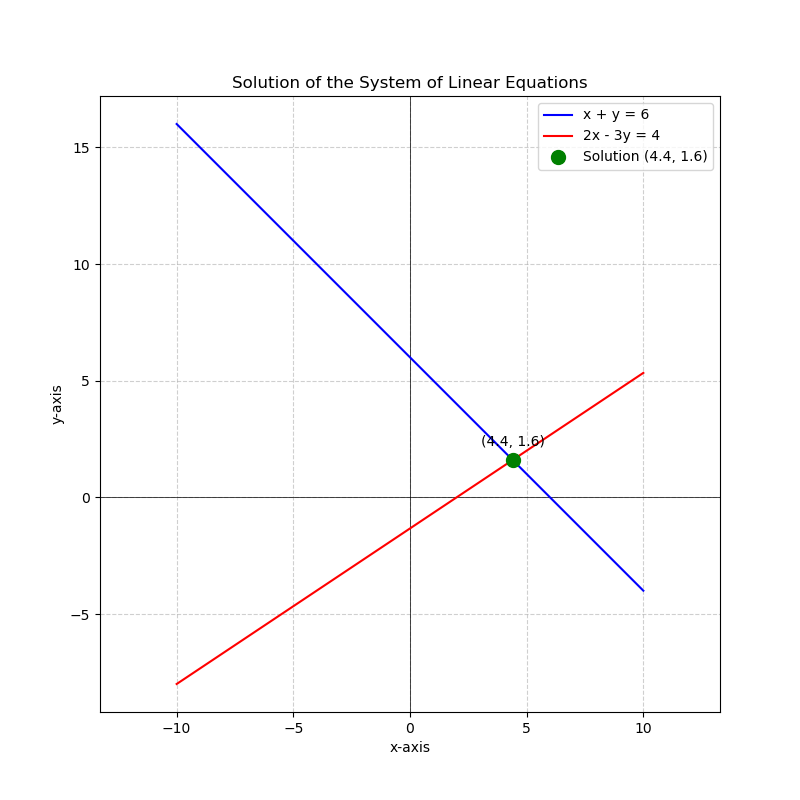
\includegraphics[width=1\linewidth]{figs/plot.png}
    \caption{}
    \label{fig:placeholder}
\end{figure}

\end{document}






